\ifdefined\included
\else
\documentclass[a4paper,11pt,twoside]{StyleThese}
\usepackage{amsmath,amssymb, amsthm}             % AMS Math
\usepackage[T1]{fontenc}
\usepackage[utf8x]{inputenc}
\usepackage{babel}
\usepackage{datetime}

\usepackage{silence}

\WarningFilter{minitoc(hints)}{W0023}
\WarningFilter{minitoc(hints)}{W0028}
\WarningFilter{minitoc(hints)}{W0030}

\usepackage{lmodern}
\usepackage{tabularx}
%\usepackage{tabular}
\usepackage{multirow}
\usepackage{xspace}

\usepackage{subfig}
\usepackage[inline]{enumitem}

\usepackage{hhline}
\usepackage[left=1.5in,right=1.3in,top=1.1in,bottom=1.1in,includefoot,includehead,headheight=13.6pt]{geometry}
\renewcommand{\baselinestretch}{1.05}

% Table of contents for each chapter

\usepackage[nottoc, notlof, notlot]{tocbibind}
\usepackage{minitoc}
\setcounter{minitocdepth}{2}
\mtcindent=15pt
% Use \minitoc where to put a table of contents

\usepackage{aecompl}

% Glossary / list of abbreviations

\usepackage[intoc]{nomencl}
\iftoggle{ThesisInEnglish}{%
\renewcommand{\nomname}{Glossary}
}{ %
\renewcommand{\nomname}{Liste des Abréviations}
}

\usepackage{etoolbox}
\renewcommand\nomgroup[1]{%
  \item[\bfseries
  \ifstrequal{#1}{A}{Number Sets}{%
  \ifstrequal{#1}{G}{Agents Beliefs and Action Models}{%
  \ifstrequal{#1}{N}{Navigation}{%
  \ifstrequal{#1}{O}{Ontology}{%
  \ifstrequal{#1}{R}{Referring Expression Generation}{%
  \ifstrequal{#1}{Z}{Controllable and Uncontrollable Agents Task Planning}{}}}}}}%
]}

\makenomenclature



% My pdf code

\usepackage{ifpdf}

\ifpdf
  \usepackage[pdftex]{graphicx}
  \DeclareGraphicsExtensions{.jpg}
  \usepackage[pagebackref,hyperindex=true]{hyperref}
  \usepackage{tikz}
  \usetikzlibrary{arrows,shapes,calc}
\else
  \usepackage{graphicx}
  \DeclareGraphicsExtensions{.ps,.eps}
  \usepackage[dvipdfm,pagebackref,hyperindex=true]{hyperref}
\fi

\graphicspath{{.}{images/}}

%% nicer backref links. NOTE: The flag ThesisInEnglish is used to define the
% language in the back references. Read more about it in These.tex

\iftoggle{ThesisInEnglish}{%
\renewcommand*{\backref}[1]{}
\renewcommand*{\backrefalt}[4]{%
\ifcase #1 %
(Not cited.)%
\or
(Cited in page~#2.)%
\else
(Cited in pages~#2.)%
\fi}
\renewcommand*{\backrefsep}{, }
\renewcommand*{\backreftwosep}{ and~}
\renewcommand*{\backreflastsep}{ and~}
}{%
\renewcommand*{\backref}[1]{}
\renewcommand*{\backrefalt}[4]{%
\ifcase #1 %
(Non cité.)%
\or
(Cité en page~#2.)%
\else
(Cité en pages~#2.)%
\fi}
\renewcommand*{\backrefsep}{, }
\renewcommand*{\backreftwosep}{ et~}
\renewcommand*{\backreflastsep}{ et~}
}

% Links in pdf
\usepackage{color}
\definecolor{linkcol}{rgb}{0,0,0.4} 
\definecolor{citecol}{rgb}{0.5,0,0} 
\definecolor{linkcol}{rgb}{0,0,0} 
\definecolor{citecol}{rgb}{0,0,0}
% Change this to change the informations included in the pdf file

\hypersetup
{
bookmarksopen=true,
pdftitle="Endowing the robot with the abilities to control and evaluate its contribution to a human-robot joint action",
pdfauthor="Amandine MAYIMA", %auteur du document
pdfsubject="Thèse", %sujet du document
%pdftoolbar=false, %barre d'outils non visible
pdfmenubar=true, %barre de menu visible
pdfhighlight=/O, %effet d'un clic sur un lien hypertexte
colorlinks=true, %couleurs sur les liens hypertextes
pdfpagemode=None, %aucun mode de page
pdfpagelayout=SinglePage, %ouverture en simple page
pdffitwindow=true, %pages ouvertes entierement dans toute la fenetre
linkcolor=linkcol, %couleur des liens hypertextes internes
citecolor=citecol, %couleur des liens pour les citations
urlcolor=linkcol %couleur des liens pour les url
}

% definitions.
% -------------------

\setcounter{secnumdepth}{3}
\setcounter{tocdepth}{2}

% Some useful commands and shortcut for maths:  partial derivative and stuff

\newcommand{\pd}[2]{\frac{\partial #1}{\partial #2}}
\def\abs{\operatorname{abs}}
\def\argmax{\operatornamewithlimits{arg\,max}}
\def\argmin{\operatornamewithlimits{arg\,min}}
\def\diag{\operatorname{Diag}}
\newcommand{\eqRef}[1]{(\ref{#1})}

\usepackage{rotating}                    % Sideways of figures & tables
%\usepackage{bibunits}
%\usepackage[sectionbib]{chapterbib}          % Cross-reference package (Natural BiB)
%\usepackage{natbib}                  % Put References at the end of each chapter
                                         % Do not put 'sectionbib' option here.
                                         % Sectionbib option in 'natbib' will do.
\usepackage{fancyhdr}                    % Fancy Header and Footer

% \usepackage{txfonts}                     % Public Times New Roman text & math font
  
%%% Fancy Header %%%%%%%%%%%%%%%%%%%%%%%%%%%%%%%%%%%%%%%%%%%%%%%%%%%%%%%%%%%%%%%%%%
% Fancy Header Style Options

\pagestyle{fancy}                       % Sets fancy header and footer
\fancyfoot{}                            % Delete current footer settings

%\renewcommand{\chaptermark}[1]{         % Lower Case Chapter marker style
%  \markboth{\chaptername\ \thechapter.\ #1}}{}} %

%\renewcommand{\sectionmark}[1]{         % Lower case Section marker style
%  \markright{\thesection.\ #1}}         %

\fancyhead[LE,RO]{\bfseries\thepage}    % Page number (boldface) in left on even
% pages and right on odd pages
\fancyhead[RE]{\bfseries\nouppercase{\leftmark}}      % Chapter in the right on even pages
\fancyhead[LO]{\bfseries\nouppercase{\rightmark}}     % Section in the left on odd pages

\let\headruleORIG\headrule
\renewcommand{\headrule}{\color{black} \headruleORIG}
\renewcommand{\headrulewidth}{1.0pt}
\usepackage{colortbl}
\arrayrulecolor{black}

\fancypagestyle{plain}{
  \fancyhead{}
  \fancyfoot{}
  \renewcommand{\headrulewidth}{0pt}
}

%\usepackage{MyAlgorithm}
%\usepackage[noend]{MyAlgorithmic}
\usepackage{algorithm}
\usepackage[noend]{algpseudocode}
\usepackage{comment}
\usepackage[ED=MITT-InfoTel, Ets=INSA]{tlsflyleaf}
%%% Clear Header %%%%%%%%%%%%%%%%%%%%%%%%%%%%%%%%%%%%%%%%%%%%%%%%%%%%%%%%%%%%%%%%%%
% Clear Header Style on the Last Empty Odd pages
\makeatletter

\def\cleardoublepage{\clearpage\if@twoside \ifodd\c@page\else%
  \hbox{}%
  \thispagestyle{empty}%              % Empty header styles
  \newpage%
  \if@twocolumn\hbox{}\newpage\fi\fi\fi}

\newcommand*{\algrule}[1][\algorithmicindent]{%
	\makebox[#1][l]{%
		\hspace*{.2em}% <------------- This is where the rule starts from
		\vrule height .75\baselineskip depth .25\baselineskip
	}
}

%%% to have lines in algorithm, from stackexchange
\newcount\ALG@printindent@tempcnta
\def\ALG@printindent{%
	\ifnum \theALG@nested>0% is there anything to print
	\ifx\ALG@text\ALG@x@notext% is this an end group without any text?
	% do nothing
	\else
	\unskip
	% draw a rule for each indent level
	\ALG@printindent@tempcnta=1
	\loop
	\algrule[\csname ALG@ind@\the\ALG@printindent@tempcnta\endcsname]%
	\advance \ALG@printindent@tempcnta 1
	\ifnum \ALG@printindent@tempcnta<\numexpr\theALG@nested+1\relax
	\repeat
	\fi
	\fi
}
% the following line injects our new indent handling code in place of the default spacing
\patchcmd{\ALG@doentity}{\noindent\hskip\ALG@tlm}{\ALG@printindent}{}{\errmessage{failed to patch}}
\patchcmd{\ALG@doentity}{\item[]\nointerlineskip}{}{}{} % no spurious vertical space
% end vertical rule patch for algorithmicx

\makeatother
 
%%%%%%%%%%%%%%%%%%%%%%%%%%%%%%%%%%%%%%%%%%%%%%%%%%%%%%%%%%%%%%%%%%%%%%%%%%%%%%% 
% Prints your review date and 'Draft Version' (From Josullvn, CS, CMU)
\newcommand{\reviewtimetoday}[2]{\special{!userdict begin
    /bop-hook{gsave 20 710 translate 45 rotate 0.8 setgray
      /Times-Roman findfont 12 scalefont setfont 0 0   moveto (#1) show
      0 -12 moveto (#2) show grestore}def end}}
% You can turn on or off this option.
% \reviewtimetoday{\today}{Draft Version}
%%%%%%%%%%%%%%%%%%%%%%%%%%%%%%%%%%%%%%%%%%%%%%%%%%%%%%%%%%%%%%%%%%%%%%%%%%%%%%% 

\newenvironment{maxime}[1]
{
\vspace*{0cm}
\hfill
\begin{minipage}{0.5\textwidth}%
%\rule[0.5ex]{\textwidth}{0.1mm}\\%
\hrulefill $\:$ {\bf #1}\\
%\vspace*{-0.25cm}
\it 
}%
{%

\hrulefill
\vspace*{0.5cm}%
\end{minipage}
}

\let\minitocORIG\minitoc
\renewcommand{\minitoc}{\minitocORIG \vspace{1.5em}}

\usepackage{multirow}
%\usepackage{slashbox}

\newenvironment{bulletList}%
{ \begin{list}%
	{\tiny$\bullet$}%
	{\setlength{\labelwidth}{25pt}%
	 \setlength{\leftmargin}{30pt}%
	 \setlength{\itemsep}{-0.5em}}}%
{ \end{list} }

\newenvironment{inlineEnumerate}
{\begin{enumerate*} [label={(\arabic*)}] }
{\end{enumerate*}}

\theoremstyle{definition}
\newtheorem{definition}{Definition}
\renewcommand{\epsilon}{\varepsilon}

% centered page environment

\newenvironment{vcenterpage}
{\newpage\vspace*{\fill}\thispagestyle{empty}\renewcommand{\headrulewidth}{0pt}}
{\vspace*{\fill}}

\newenvironment{asl}{\ttfamily\begin{tabbing}~~~\=$\leftarrow$ \= ~~~ \=
		\kill}{\end{tabbing}}

\usepackage{tablefootnote}

\theoremstyle{plain}
\newtheorem{constraint}{Constraint}[section]

\algnewcommand\algorithmicforeach{\textbf{for each}}
\algnewcommand\algorithmicin{\textbf{in}}
\algdef{S}[FOR]{ForEach}[2]{\algorithmicforeach\ #1\ \algorithmicin\ #2\ \algorithmicdo}

\algnewcommand\algorithmicforkxor{\textbf{do fork-join-xor}}
\algnewcommand\algorithmicendforkxor{\textbf{end fork-join-xor}}
\algdef{SE}{ForkXor}{EndForkXor}{\algorithmicforkxor}{\algorithmicendforkxor}


\usepackage{listings}
\lstset{
	frame=single,
	captionpos=b,
	breaklines=true,
	basicstyle=\ttfamily,
	numberstyle=\color{black},
	tabsize=2,
	mathescape=true,
	literate=%
		{â}{{\^a}}1
}

\lstdefinestyle{inline}{
	frame=none,
	aboveskip=\smallskipamount,
	belowskip=\smallskipamount,
}

\lstdefinestyle{OwlTurtle}{
	language=C,
	tabsize=4,
	basicstyle=\scriptsize\ttfamily,
	keywordstyle=\bfseries\color{darkgray},
	morekeywords={rdf:type, rdfs:domain, rdfs:subPropertyOf, rdfs:range, :hasSubtask, :DecompositionUsedBy, rdfs:subClassOf, :hasDecomposition, owl:inverseOf, htn_actions:hasEffect, rdfs:label},
	alsoletter=:
}

\lstdefinestyle{aslDef}{
	frame=none,
%	breaklines=false,
	%xleftmargin=.1\textwidth, xrightmargin=.1\textwidth
}

\fancypagestyle{example}{%
	\fancyhead[LE]{\bfseries\thepage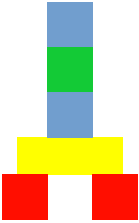
\includegraphics[scale=0.20]{figures/chapter2/task_goal.pdf}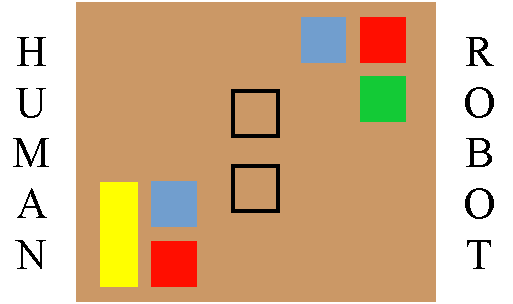
\includegraphics[scale=0.18]{figures/chapter2/task_setup_mini.pdf}}   
	\fancyhead[RO]{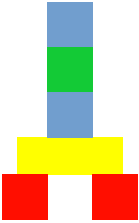
\includegraphics[scale=0.20]{figures/chapter2/task_goal.pdf}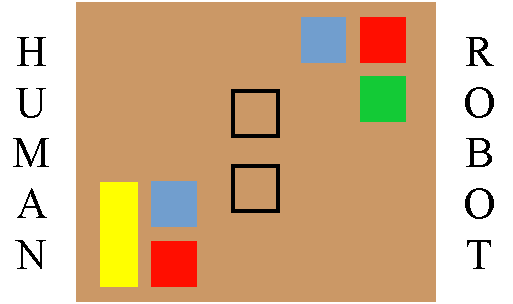
\includegraphics[scale=0.18]{figures/chapter2/task_setup_mini.pdf}\bfseries\thepage}  
	\fancyhead[RE]{\bfseries\nouppercase{\leftmark}}      % Chapter in the right on even pages
	\fancyhead[LO]{\bfseries\nouppercase{\rightmark}}     % Section in the left on odd pages
}%

\usepackage{pdfpages}
\usepackage{makecell}
\usepackage{pdflscape} 
\usepackage{mathtools}
\usepackage[section]{placeins}
\usepackage{afterpage}

%%%%%%%% my commands
\newcommand{\etal}{\textit{et al}.}
\newcommand{\ie}{\textit{i.e.}, }
\newcommand{\eg}{\textit{e.g.}, }
\newcommand{\fact}[3]{\mbox{\textit{#1}(#2, #3)}}
\newcommand{\circledtext}[1]{\raisebox{.5pt}{\textcircled{\raisebox{-.9pt} {#1}}}}
\newcommand{\sparql}{\textsc{SPARQL}}

\newcommand{\algConst}[1]{${\scriptscriptstyle #1}$}
\newcommand{\algNormTextSub}[2]{$\text{#1}_{#2}$}

\newcommand{\aslnumber}[1]{$#1$}
\newcommand{\aslstring}[1]{\textsf{#1}}
\newcommand{\aslvar}[1]{\textcolor{purple}{\textit{#1}}}
\newcommand{\asllabel}[1]{\textbf{#1}}
\newcommand{\annotation}[1]{{\footnotesize #1}}
\newcommand{\rulebody}[1]{\mbox{\hspace{.05\linewidth}}\begin{minipage}[t]{0.9\linewidth}#1.\end{minipage}}
\newcommand{\context}[1]{\begin{minipage}[t]{0.9\linewidth}#1\end{minipage}}
\newcommand{\planbody}[1]{\begin{minipage}[t]{0.9\linewidth}#1.\end{minipage}}
\newcommand{\Jason}[0]{\textbf{\textit{Jason}}}
\newcommand{\sn}{\mbox{\large\textbf{\texttt{\textasciitilde}}}}


\sloppy
\begin{document}
\setcounter{chapter}{0} %% Numéro du chapitre précédent ;)
\dominitoc
\faketableofcontents
\fi

\chapter{Human, Robot and Interaction Models: the Funding Principles of a Decision-Making System for Human-Robot Collaboration}
\label{chapter:chap1}
\chaptermark{Human, Robot and Interaction Models}
\minitoc

This first chapter aims at setting the context for this thesis. First, we present some related works on human-human and human-robot social interactions. These works nourished the thoughts which led to this manuscript. Then, we develop key elements for collaboration such as joint action, commitment and shared plans. Finally, we explore \acrfull{bdi} and cognitive robotic architectures  which have inspired us to design our own architecture in which, \acrshort{jahrvis} —  the main contribution of this thesis — endows a robot with the abilities not only to control, but also to evaluate its joint action with a human. 


\section{Social interactions}\label{sec:soc_int}\todo{check refs to CA}

\subsection{How to define a social interaction?}
First, let’s take a look at the dictionary and see how the word ``interaction'' is defined. According to the Oxford dictionary, an interaction is a ``reciprocal action or influence'' and more precisely a ``communication or direct involvement with someone or something''. As for the Cambridge dictionary, it defines it as an occasion when two or more people or things communicate with or react to each other''. Those definitions can give an hint about what it an interaction between humans but they are not specific enough. Now, going through social psychology literature, one of the first attempt to define ``social interaction'' can be found in~\cite{goffman_1967_interaction}. Goffman distinguishes three basic interaction units: the social occasion, the gathering and the social situation. The social occasion is an event that is temporally and spatially situated in such a way that it forms a unit that can be looked forward and back upon, by participants that are informed by the event (dinner, meeting, sport game...).  The gathering refers to any set of two or more individuals who are at the moment in one another’s immediate presence. It can be noted that a social occasion may include several gatherings but that gathering do not need social occasions to occur (they can happen in office spaces, street corners, restaurants…). The social situation refers to the full spatial environment that embraces interacting people. It is created as soon as people engage in interaction, when mutual monitoring occurs and ends when the next to the last person leaves. Furthermore, Goffman distinguishes between focused and unfocused interaction (gathering). A focused gathering has its members that can come together to sustain a joint focus of visual and cognitive attention and are open to each other for talk. He calls it encounters or engagements. On the other hand, an unfocused gathering has its members present to one another but not engaged together (e.g. persons waiting for a bus). In this same book, Goffman proposes a definition of social encounter: ``an occasion of face-to-face interaction, beginning when individuals recognize that they have moved into one another’s immediate presence and ending by an appreciated withdrawal from mutual participation''.

A couple of years later, Argyle wrote a book entitled Social Interaction~\cite{argyle_1973_social}, where he lay the foundations the basis to understand social interactions. He came to the view that social interaction could be interpreted as a set of social skills, and that it may therefore be possible to train those skills as manual skills are trained. For example, during an encounter between two persons, each must be able to perceive the social cues (verbal or non-verbal signals) of the other which are then filtered through the perspective each has acquired through socialization and experience.  The interpretation of context and social cues is then applied to arrive at a definition of the situation, which in turn guides both behavior and action.

Then, \cite{rummel_1976_understanding} proposes a definition of a few words: ``Social interactions are the acts, actions, or practices of two or more people mutually oriented towards each other's selves. It is behavior that tries to influence or take into account another's subjective experiences or intentions''.

Finally, the elements brought here, trying to define what is an interaction and more precisely a social interaction, are chosen among a large amount of work. It is possible to find different definitions, as \cite{enriquez_2017_vocabulaire} precises: ``although the term ``interaction'' is frequently used, it does not have a unique definition but presents semantic divergences''.

\subsection{Structure of a social interaction}
Most of the research about interaction and social interaction belongs to the field of social psychology. As for the structure of a social interaction, it is more from the field of Conversation Analysis (CA) which mixes sociology, anthropology, linguistics, speech-communication and psychology.
In~\cite{robinson_overall_2012}, Robinson makes a review of the work that has been done about ``overall structural organization''. Most of the time in the literature, overall structural organization is discussed in terms of ``the overall structural organization of entire, single occasions of interaction''.  Then ``overall structural organization'' term is generally used to talk about one particular (albeit large) unit of interaction. However, many different types of interactional units can have an overall structural organization. For example, in~\cite{schegloff_2011_word}, Schegloff encourages to recognize ``‘overall structural organization’ not as something for the unit ‘a single conversation’ (or encounter, or session, etc.) alone, but for units like turns, actions and courses of action (like answering or telling), sequences, and who knows what else as well.'' He also mentioned that every unit of organization should probably have a local organization and a global organization.
Here, the term ``overall structural organization'' is to refer to ``the overall structural organization of entire, single occasions of interaction''. Robinson tells us that this concept has received relatively little analytic attention and thus is still not well understood~\cite{robinson_overall_2012}. Indeed, research has been more focused on analyzing the organization of individual sequences of action such as turn-takings or conversation openings. Several terms have been used to talk about a ``supra-sequential coherence'': big package, set of pre-organized sequences, (social) activity, project of activity or plan of action. As the subject has not been investigated so much, it has not evolved a lot in 40 years, since what was proposed by Sacks~\cite{sacks_lectures_1995} to define overall structural organization of single occasions of interaction: it ``deals, roughly, with beginnings and endings, and how beginnings work to get from beginnings to something else, and how, from something else, endings are gotten to. And also the relationship - if there is one - between beginnings and endings''. Robinson summarizes research about the subject by saying that single occasions of interaction (in a generic or context-free sense) are normatively organized as: (1) beginning with an opening (2) ending with a closing and (3) having ``something'' in between opening and closing'' which can be referred to as topics.

\subsubsection{Opening}
Openings are used to begin an encounter. One of the main reference on the subject is~\cite{schegloff_1986_routine}. Openings and related issues vary depending on the nature of interactions. For example, opening of a phone call to a family member or a friend will be organized as follow: (1) summons-answer (the one calling talks first) (2) identification/recognition of each other (3) greetings and (4) how-are-you. Whereas, in primary-care medical visits, opening is sequenced as: (1) greeting (2) securing patients’ identities (2) retrieving and reviewing patients’ records and (4) embodying readiness (sitting down and facing one another). More examples from the literature can be found in (Robinson, 2012). 

Another work, \cite{kendon_1990_conducting}, focuses on the greeting part, but more precisely the greeting behavior with the associated non-verbal cues. The greeting behavior is divided in three main phases: the distance salutation, the approach and the close salutation. 
The distance salutation only occurs if the greeters as far enough such as they need to get closer if they wish to continue the interaction. This phase starts after one or both participants sight one another and at least one of them identifies a wish to engage in a greeting. In case one of the participant has not seen the other one, he signals his presence by vocalizing the other one’s name or by clearing his throat. Then, they orient their bodies towards each other and exchange glances in a subtle acknowledgement that the greeting is desired by both. During this phase, people can also wave or give a sign with their head (e.g. nod).
The approach is divided into two sub-phases: the distant approach (Kendon does not use this term) and the final approach. During the distant approach, people tend to look away whereas when the final approach starts (the greeters are 3 meters or less from one another), they look back at each other and, they smile.
Finally, there is the close salutation, the most normalized phase of the greeting. It happens when people are 1,5 meters or less from each others. Then, they can have a non-contact close salutation during which people exchange verbal greetings, or they can hand-shake or embrace (or do something else according to their culture). The greeting is over.
\subsubsection{Topics}
Episodes of interaction vary a lot in their contextualized nature, which leads to a large variety of topics and sequences of topics. Interactions that happen in ordinary or institutional contexts can be pre-organized around one or more topics. Robinson give examples such as an emergency call or an expected call back by a friend to discuss an expected single item of business.

\subsubsection{Closing}
One of the main reference to talk about closings is~\cite{schegloff_1973_opening}. A closing can be divided into two phases: the topic termination and the leave-taking.
The topic termination has a pre-closing statement which signals to the partner the wish to close the conversation. Then, the leave-taking follows the pre-closing statement and its response and, includes the goodbye exchange. Finally, the partners break co-presence, \ie, physically walk apart.\footnote{It is not explicitly mentioned in~\cite{schegloff_1973_opening}  but they precise in a footnote that it would not make sense if the parties remain in co-presence after having being through the closing sequence.} In the context of a phone call, Clark and French define this co-presence breaking as the \textit{contact termination} when people hang up.

With regards to non-verbal cues,  Knapp \etal lists and analyzes them~\cite{knapp_1973_rhetoric}. The more frequent are eye contact breaking,  head nodding, leaning toward the partner and positioning in the direction of the way of leaving.

\section{Human-Robot Social Interactions}

Now that we have seen how social interactions look like when happening between humans, we are going to see the different ways the human-robot interaction field divided and categorized interactions. 

\subsection{Short-term Interactions}
In~\cite{zheng_2013_designing}, they define a ``short-term interaction'' based on the Unified Theories of Cognition of Newell~\cite{newell_1994_unified}. A short-term interaction corresponds to the ``cognitive band'' of cognition, during which they focus on individual utterances and speech acts for interactions that last for tens of seconds. They leave aside longer-term interactions that can be in the ``rational band'' (minutes to hours) or the ``social band'' (days to months).
In~\cite{gaschler_2012_modelling}, their robot is a bartender then, they define a short-term interaction as being a customer ordering a drink – from the attention request towards the bartender to the closing of interaction by payment and exchange of polite phrases.
In~\cite{iocchi_2015_personalized}, they use ``short-term'' to refer to short interactions and that are focused on only one particular communicative objective, avoiding long and complex interactions.
In~\cite{sanelli_2017_short}, they give three characteristics to a short-term human-robot interaction: (1) users are not familiar with the robot (2) each interaction happens with a different user (3) interaction is short in time. Then the robot has not memory of past interactions.

\subsection{Long-term Interactions}
A survey~\cite{leite_2013_social} has been done about long-term human-robot interactions, where long-term means, most of the time, several interactions between the same human and robot. They defined four contexts for which social robot\footnote{actually, some of the robots featured in the survey are not social robots such as a Roomba or the Personal Exploration Rover (PER)} for long-term interaction have been designed: health care and therapy, education, work environment and public spaces, and people's homes. 
For example, Kanda \etal performed a field trial at an elementary school in Japan for two months~\cite{kanda_2007_two}. The children were able to interact with the robot for 32 days in total, during 30 minutes after lunch. The robot could switch between one hundred pre-defined behaviors (\eg hugging, shaking hand or singing) but not all of them were available during the first interactions with a human. Indeed, they had integrated a pseudo-development mechanism, \ie the more a child interacts with the robot, the more different behaviours the robot displays to that child. Also, the robot confided personal-themed matters to children who have often interacted with it (\eg ``I don't like the cold''). These abilities allowed the robot to maintain the children's interest even after the first week whereas in a first experiment where the robot's behavior was the same all along the two months, most children stopped to interact with the robot from the second week. 

In their discussion part, they raise an interesting question: How Long Should ``Long-Term'' Be? They found out that some authors consider that two months is a long-term interaction. They also point that some Human-Computer Interaction studies on long-term interaction last five weeks. Finally, the authors of the survey give their point of view, which seems well-thought. They argue that it is more important to look at the number of interaction sessions and the length of these sessions (a five minutes-interaction is different from a one hour-interaction). For them, an interaction can be considered as ``long-term'' when the user becomes familiarized with the robot to a point that their perception of such robot is not biased by the novelty effect anymore. This definition raises another question: when does user’s familiarization with the robot become stable? But it is not discussed here.

\subsection{Interactions divided in phases}
Among works on short-term or long-term interactions, some authors divide interactions in phases which have sometimes similarities with the phases of social interactions described in Section~\ref{sec:soc_int}.

Gockley \etal divide an interaction in three phases: greeting, core of the interaction and departure~\cite{gockley_2005_designing}. In the greeting phase, Valerie, the robot receptionist, greets people who might be interested in engaging in conversation. To do so, people are classified into ``attentional'' states:
\begin{enumerate*}
	\item present (people a bit far and moving): Valerie doesn’t pay attention to them
	\item attending (people closer): Valerie greets them
	\item engages (people next to the desk but on the side): Valerie acknowledges their presence but does not expect input from them
	\item interacting (people in front of the keyboard): Valerie prompts them for input if they are not typing.
\end{enumerate*}
In the core of interaction, either Valerie can tell her (fictive) story or chat. Her story is subjective and evolve over time. It is about her social life, her lounge singing career, her therapy business, and her job as a receptionist. Furthermore, Valerie has a chatbot system which is very simple. Finally, inputs from visitors are from a keyboard, for easier control and reliability. Finally, at departure, when a person leaves the ``interacting'' region, Valerie signals the end of the interaction by saying ``goodbye.'' 

In~\cite{kidd_2008_robots}, they present a weigh loss coach. It introduces the notion of states of relationship. They are three: initial (for the first few days of interaction), normal, repair. According to the state of relationship, the robot answers/questions/speech will not be the same.

In~\cite{kasap_2012_building}, to each user, corresponds an interaction session. Each session is composed of four dialogue phases: welcome, warm up, teach and farewell. The system has a memory of users and past interactions. In the memory, is recorded the context (initial state and goal), contents (events) and the outcome (goal succeeded or not).  A bit similar to the relationship state defined in~\cite{kidd_2008_robots}, they define a notion that they call relationship level. It is computed from the emotional interactions from the episodic memory associated to a user. It will influence the mood level and then the facial expression and the speech.

In~\cite{gaschler_2012_modelling}, they divide the interaction in three phases (or states) but from two different viewpoints, the of the customer and the one of the bartender. From the customer viewpoints, the phases are: (1) attention request towards bartender (2) ordering of one or more beverages, and (3) closing of interaction by payment and exchange of polite phrases. Then, in reaction of each phases, there are the ones from the bartender viewpoint: (1) acknowledging the attention request, (2) serving the ordered drink, and (3) asking for payment.
They leave open the possibility to have sub-phases inside phases.

We can also find in~\cite{lee_2012_personalization} the notion of structure of interaction: interactions start with the vendor identifying the customer, greeting and engaging in small talk with the customer, engaging in the snack transaction, and then enacting social leave-taking.

\subsection{Hierarchical interactions}
Not only, interactions can be divided in phases but also in levels. In~\cite{dautenhahn_2002_embodied} and~\cite{ogden_2001_interactional}, they define two levels of approach for interactions, a global one and a local one. Both papers are from the same authors but present some small differences in their definitions of the levels.
In~\cite{dautenhahn_2002_embodied}, the global level approach defines a unit of interaction as being relatively large, such as the script for a greeting as described by Kendon in~\cite{kendon_1990_conducting}. At this level, an interaction may be seen as a unit similar to a schema or script, in the computer/cognitive science senses of these terms. They name this level of interaction a Global Interactional Unit (GIU). Furthermore, a GIU can be divided in phases, each of which has associated behaviors. Behaviors have meaning and their meaning depends on the phase in which they occur, the context (e.g. a ‘wave hello’ vs. a ‘wave goodbye’). Finally, they discuss the advantages and drawbacks to describe an interaction at a global level. In~\cite{ogden_2001_interactional}, they prefer the use of the term ``long sequences of interaction'' rather than ``large units of interaction''.
In~\cite{dautenhahn_2002_embodied}, their local level approach is quite similar to the way CA views and analyzes interaction (e.g. adjacency pairs). This interactional structure is a much smaller unit, often as simple as an action and a response to that action. This view of interaction has the advantage of greater flexibility and robustness compared to the globally structured view. Flexibility is a result of the possibility of specifying acts that may occur in many global interactional structures. But, as contextual details are ignored, the ability to assign a specific meaning to an action is lost.

In his thesis, Kuo insists about this flexibility and the re-usability~\cite{kuo_2012_designing}. A lower level of design is more appropriate for reuse. For him, a unit of interaction corresponds to an ``interaction cue'' (or social cue) that a robot can perceive and act upon or express in an interaction. These cues can be verbal, non-verbal, or a combination of both (multi-modal interaction). A complete episode of interaction should be constructed through composition of interaction cues with some common patterns repeated over the course of the interaction (e.g. awareness of human presence).

\subsection{Patterns of Interaction}
Before talking about design patterns or interaction patterns, Goffman in 1983~\cite{goffman_1983_interaction} argues that human interactions follow a specific ``order'' and characterized a number of patterns in which people interact, such as how greetings unfold and how people leave an interaction.

In!\cite{kahn_2008_design}, they introduce design patterns, that they will later called interaction patterns in~\cite{kahn_2010_validating}, inspired from computer science. They propose rules to follow using them and eight patterns. The two main ideas to retain is that a sequence of patterns has to be well ordered and that patterns can be hierarchical. 
The 8 patterns: 
\begin{enumerate*}
	\item The initial introduction: largely scripted, conventionally-established verbal and behavioral repertoire to recognize the other, inquire politely about the other, engage in some physical acknowledgment (e.g. handshake)
	\item Didactic communication: one-way communication of information 
	\item In motion together: walk together
	\item Personal interests and history: sharing of personal interests and history with others
	\item Recovering from mistakes: creates the potential for both parties to maintain a social affiliation following the mistake
	\item Reciprocal turn-taking in game contextual: taking turns with one another when playing games
	\item Physical intimacy: to engage in holding or touching or embracing
	\item Claiming unfair treatment or wrongful harms: allows to make claim to its moral standing
\end{enumerate*}


Following the same idea and going further, Sauppé and Mutlu~\cite{sauppe_2014_design} introduces the interaction blocks. Compared to Kahn’s work, they offer a pattern language and a tool/environment to design human-robot interaction. To conceive their patterns, they collected and analyzed data from 5 kinds of interaction scenarios: Conversation, Collaboration, Instruction, Interview and Storytelling.
Then, they identified common interaction structures, which served as ``design interaction patterns'':
\begin{enumerate*}
	\item Introductory monologue: A short introduction can be used to introduce other participants to a scenario by giving an overview of the remainder of the interaction or it can be a greeting for example.
	\item Question and Answer: A question is a sentence meant to elicit information from other participants. An answer is the response to a question that aims to satisfy the questioning participant’s curiosity.
	\item Generic Comment and Personal Comment: A comment is a short statement offering the speaker’s opinion. Comments are either generic (e.g., ``Wow'') or personal (e.g., ``I tried that and didn’t like it'').
	\item Monologue and Generic Comment: A monologue is a longer form of speech during which no response is expected.(e.g. telling of a story). Although monologues expect no response, listeners may occasionally offer unsolicited commentary.
	\item Instruction and Action: An instruction is a command offered by one participant to direct the actions of another participant. The proper response to this instruction is often an action, although the action might follow the instruction with a delay depending on whether it is an appropriate time to perform that action
	\item Finished Comment: Upon the completion of the goals of the scenario, one or more of the participants will note that the scenario is completed by offering a finished comment.
	\item Wait: One pattern implicit in all scenarios involving two or more participants is the wait pattern.
\end{enumerate*}
Finally, they designed a software to easily implement those patterns in a robot.

In his thesis~\cite{kuo_2012_designing}, Kuo criticizes Kahn’s work. He says that these patterns involve sequences of interaction cues and should be decomposed to a lower level for detailed design and reuse. He proposes his own patterns:
\begin{enumerate*}
	\item Human presence detection: detect when there is a person who might be interested in
	\item Showing interest for interaction: express the robot’s awareness of a user’s presence around it and its interest and willingness to interact
	\item User’s attention on the robot: Know when a user is paying attention to the robot in an interaction and its information on its screen
	\item User identification by face: Provides the fundamental block for personal service and social interaction by recognising the human counterpart in an interaction
\end{enumerate*}
He checked the validity of his patterns with the analysis of Problem statement, Context of Use, Interaction Modality, Combination with Other Patterns, Technical Performance and Limitations, User Feedback and User’s Perception, Resulting Interactive Behavior.

Finally, Peltason and Wrede also based their work on design patterns from computer science, specifically applied to dialogue here~\cite{peltason_2010_pamini}. To name a few of them: Simple action request, Interaction opening, Interaction closing, Clarification. During interaction, the registered patterns are employed in a flexible way by admitting that patterns can be interrupted by other patterns and possibly resumed later which leads to interleaving patterns. By default, simpler patterns are permitted to be nested within temporally extended patterns.

\section{Around the Joint Action Concept}
Often, multiple concepts are addressed when referring to collaborative tasks: collaboration, cooperation, coordination, joint action, joint activity, shared/joint attention, shared/joint intention, shared plan, shared/common/joint goal, (joint) commitment, engagement, mental states, theory of mind, mutual knowledge. However, many terms and definitions, whether inside a field\footnote{Here, philosophy, psychology or robotics} or between fields do not reach a consensus. This can be quite confusing, especially for roboticists for which it is not the range of expertise at first.

\subsection{How to define Joint Action ?}

An important number of social interactions and encounters are encompassed by the notion of joint action. Broadly considered, joint action is any form of social interaction whereby two agents or more coordinate their actions in order to pursue a joint goal. However, the notion of joint action has particularly been subject to debate in philosophy and psychology. For instance, according to Sebanz \etal~\cite{sebanz_2006_joint}, ``joint action can be regarded as
any form of social interaction whereby two or more individuals coordinate their actions in space and time to bring about a change in the environment.'' (p. 70); while other authors~\cite{carpenter_2009_just, cohen_1991_teamwork\todo{à laisser ? mecs de l'IA ?}, fiebich_2013_joint, tomasello_2005_understanding} resist the idea that instances of mere coordination  – e.g. two partners walking side by side – constitute a joint action, considering that it requires some necessary conditions like sharing goals and intentions.

Moreover, while the notion of joint action is used interchangeably with the notion of collaboration or cooperation for some authors such as Becchio \etal~\cite{becchio_2010_toward} and Kobayashi \etal~\cite{kobayashi_2018_language}, other authors establish a hierarchy of interactions depending on the processes involved~\cite{amici_2015_coordination, chalmeau_1995_cooperation}. According to Amici and Bietti~\cite{amici_2015_coordination}, for example, coordination is a fast low-level process of behavioral matching and interactional synchrony which could, but not necessarily, facilitate middle-level processes like cooperation (where some individuals bear certain costs to provide benefits to others) or high-level processes like joint action, which requires other resources like turn-taking and alignment of linguistic resources during dialogue.

If we look at Sebanz and colleagues definition of joint action, it could be considered as a kind of activity based on the usual sense of this term. Thus, some authors use the concept ``joint activity'' interchangeably with ``joint action''~\cite{tollefsen_2005_let,grafenhain_2013_three} while others see the joint activity composed of joint actions~\cite{clark_1996_using, feltovitch_2005_common}. Clark says that ``Joint activities advance mostly through joint actions''. He defines the properties of a joint activity among which there are: it is carried out by 2 or more participants, each participant has a public role or they try to establish and achieve joint goals, and they may have private goals. He also highlights the need for coordination. 

\subsection{What is necessary for Joint Action ?}

Leaving aside the debate on the concept of joint action, we aim to focus on the mechanisms that enable the consecution of joint actions. Three interrelated mechanisms appear to be key conditions for joint action: coordination, planning, and motivational alignment, each of them being supported by other processes. There has been an important deal of conceptual and empirical work investigating these processes~\cite{knoblich_2011_joint, pacherie_2012_agency}, from the sharing of a common ground to the anticipation of a partner’s actions by way of emergent coordination~\cite{curioni_2019_joint}. 

Most of all, joint actions require individuals to anchor their plans in the actual situation and generate particular coordinated actions~\cite{knoblich_2011_joint, vesper_2011_making}. This coordination can rely on different mechanisms, which are not necessarily intentional, including for example perception-action matching~\cite{brass_2001_movement}, perception of joint affordances~\cite{ramenzoni_2008_short}, joint attention~\cite{sebanz_2006_joint}. As for intentional coordination – sometimes referred to as planned coordination~\cite{curioni_2019_joint} –, it requires the partners: (i) to represent their own and others' actions, as well as the consequences of these actions, (ii) to represent the hierarchy of sub-goals and sub-tasks of the plan, (iii) to generate predictions of their joint actions, and (iv) to monitor the progress toward the joint goal in order to possibly compensate or help others to achieve their contributions~\cite{pacherie_2012_agency}.

Indeed, joint action often involves planning several aspects, which involves the representation of the goal and the whole plan, and/or even the sequence of actions to be performed. The formation of these types of representations could rely on different mechanisms, which include high-level processes such as theory of mind, team reasoning, or verbal negotiation~\cite{bratman_2013_shared} or more low-level processes as minimally representing the joint action goal and knowing that it will be achieved with others~\cite{vesper_2010_minimal}. An example of the mechanisms involved in planning a joint action is task co-representations, which allows individuals to represent the details of each other’s task. 

These representations allow individuals to generate predictions about the other’s actions, which in turn facilitate the adjustment and coordination between the partners. Interestingly, individuals can also facilitate the others’ and their own predictions by communicating relevant and reliable information for joint action. The objective is to make actions more transparent and predictable so that the decision-making on the interaction can be fluent and successful. Thus, participants in joint action often negotiate on the fly the sub-tasks, sub-goals, or ways to proceed regarding the collective task through different explicit exchanges~\cite{clark_1996_using}.



\section{Human-Robot Joint Action}\todo{part on emotions}


\subsection{Focus on Communication in Human-Robot in Joint Action}

Cohen and Levesque, Teamwork, p 490

\subsection{Focus on Repairs in Human-Robot Joint Action}

One last subject of CA could be interesting for our problematic in human-robot interaction, it is the repair. It is a mean of correcting a misunderstanding or a mistake in an interaction, or of correcting a deviation from the normal rules of interaction. The ability to engage in repair is essential in interaction: errors and misunderstandings are likely to arise and must be corrected if the  goal of the interaction is to be successful. Generally, they are classified in four categories \cite{schegloff_1977_preference,wooffitt_2008_conversation}:
\begin{itemize}
	\item Self-initiated self-repair: Repair is both initiated and carried out by the responsible of the trouble
	\item Other-initiated self-repair: The responsible of the trouble takes care of the repair himself but the trouble have been pointed out by the other
	\item Self-initiated other-repair: The responsible of the trouble signals that a repair is needed and get the other one to repair (e.g. he forgot a name and asks for help to remember)
	\item Other-initiated other-repair: The one not responsible of the trouble initiates and carries out the repair. This is closest to what is conventionally understood as ``correction''.
\end{itemize}

\subsection{Focus on Commitments in Human-Robot in Joint Action}


\section{Supervision systems for Decision and execution}

\subsection{BDI architectures}
There are several kind of integrated cognitive architectures, a survey describes the most known and representative of them~\cite{chong_2007_integrated}. Some of them have their roots in classical artificial intelligence as the Soar architecture. Others take their inspiration in cognitive psychology as ICARUS \todo{ref} which tries to produce artificial intelligence mimicking human cognition or the BDI architecture which is based on the studies of folk psychology and intentional systems. Furthermore, inspired by neurology, there is the subsumption architecture. It is a reactive architecture therefore, it is not based on symbolic mental representations but on sensory information fusion to select actions to execute. Finally, at the crossroads between AI, cognitive psychology and neurology, we can find the ACT-R\todo{ref} and CLARION\todo{ref} models.	
The BDI model is based on the philosophical model of human practical reasoning developed and designed by Michael Bratman~\cite{bratman_1987_intention,bratman_1988_plans}. It has 3 main concepts:
\begin{itemize}
	\item Beliefs: They are a representation of the agent’s knowledge about the world. ``[They] can be viewed as the informative component of system state''~\cite{rao_1995_bdi}. It is not the word ``knowledge'' that has been chosen to define this concept because what the agent perceives of the environment is in fact the likely state of the environment. There is no certainty, its sensors are not accurate or could malfunction. This way of distinguish knowledge and beliefs is one that can be found in the literature of distributed computing~\cite{lamarre_1994_knowledge}.
	\item Desires\footnote{In one of the first implementation, PRS, ``Goals'' notion was used instead of ``Desires''~\cite{georgeff_1989_decision}, then they use it in a interchangeable way in~\cite{georgeff_1991_modeling} and finally choose ``Desires''~\cite{rao_1995_bdi} with the definition given in the AI literature, \eg desires can be many at any instant and may be mutually incompatible. Therefore, a goal will be a chosen desire~\cite{cohen_1990_intention} and concurrent goals are consistent.}: They are a representation of the motivational state of the system. They provide ``information about the objectives to be accomplished or, more generally, what priorities or payoffs are associated with the various current objectives''~\cite{rao_1995_bdi}. 
	\item Intentions: They are a representation of the currently chosen course of action (plan). It is the deliberative component of the system. The selected course(s) of action are determined with a deliberative function, according to the beliefs and desires~\cite{rao_1995_bdi}.
\end{itemize}
\subsection{Supervision for Human-Robot Interactions}

\section{Limitations and Challenges}




\ifdefined\included
\else
\bibliographystyle{acm}
\bibliography{These}
\end{document}
\fi

